\documentclass[a4paper,14pt]{extreport} % формат документа

\usepackage{amsmath}
\usepackage{cmap} % поиск в ПДФ
\usepackage[T2A]{fontenc} % кодировка
\usepackage[utf8]{inputenc} % кодировка исходного текста
\usepackage[english,russian]{babel} % локализация и переносы
\usepackage[left = 1.5cm, right = 1cm, top = 2cm, bottom = 2 cm]{geometry} % поля
\usepackage{listings}
\usepackage{graphicx} % для вставки рисунков
\usepackage{amsmath}
\usepackage{float}
\usepackage{multirow}
\usepackage{longtable}
\usepackage{array}
\graphicspath{{img/}}
\DeclareGraphicsExtensions{.pdf,.png,.jpg}
\newcommand{\anonsection}[1]{\section*{#1}\addcontentsline{toc}{section}{#1}}

\lstset{ %
	language=Lisp,                % Язык программирования 
	numbers=left,                   % С какой стороны нумеровать          
	frame=single,                    % Добавить рамку
}

\begin{document}
\begin{titlepage}

    \begin{table}[H]
        \centering
        \footnotesize
        \begin{tabular}{cc}
            \multirow{8}{*}{
\includegraphics[scale=0.35]{bmstu.jpg}}
            & \\
            & \\
            & \textbf{Министерство науки и высшего образования Российской Федерации} \\
            & \textbf{Федеральное государственное бюджетное образовательное учреждение} \\
            & \textbf{высшего образования} \\
            & \textbf{<<Московский государственный технический} \\
            & \textbf{университет имени Н.Э. Баумана>>} \\
            & \textbf{(МГТУ им. Н.Э. Баумана)} \\
        \end{tabular}
    \end{table}

    \vspace{-2.5cm}

    \begin{flushleft}
        \rule[-1cm]{\textwidth}{3pt}
        \rule{\textwidth}{1pt}
    \end{flushleft}

    \begin{flushleft}
        \small
        ФАКУЛЬТЕТ
        \underline{<<Информатика и системы управления>>\ \ \ \ \ \ \ 
        \ \ \ \ \ \ \ \ \ \ \ \ \ \ \ \ \ \ \ \ \ \ \ \ \ \ \ \ \ \ \ 
    \ \ \ \ \ \ \ \ \ \ \ \ \ \ \ } \\
        КАФЕДРА
        \underline{<<Программное обеспечение ЭВМ и
        информационные технологии>>
        \ \ \ \ \ \ \ \ \ \ \ \ \ \ \ \ \ \ \ \ }
    \end{flushleft}

    \vspace{2cm}

    \begin{center}
        \textbf{Лабораторная работа № 9} \\
        \vspace{0.5cm}
    \end{center}

    \vspace{4cm}

    \begin{flushleft}
        \begin{tabular}{ll}
            \textbf{Дисциплина} & Компьютерные сети.  \\
            \textbf{Тема} & Изучение технологии виртуальных локальных сетей (VLan)  \\
            & в сетевом симуляторе. Настройка маршрутизации между VLan.  \\
            \\
            \textbf{Студент} & Сиденко А.Г. \\
            \textbf{Группа} & ИУ7-73Б \\
            \textbf{Вариант} & 18\\
            \textbf{Преподаватель} & Рогозин Н.О.  \\
        \end{tabular}
    \end{flushleft}

    \vspace{4cm}

   \begin{center}
        Москва, 2020 г.
    \end{center}

\end{titlepage}

Для локальной общей сети был выделен частный адрес \textbf{127.168.18.0/24}. 

\begin{enumerate}

\item Назначить адреса подсетей.

Примеры назначенных IP-адресов для каждой подсети, приведены на рисунках 2-4. Общая схема приведена на рисунке 1.

\begin{figure}[H]
  \centering
  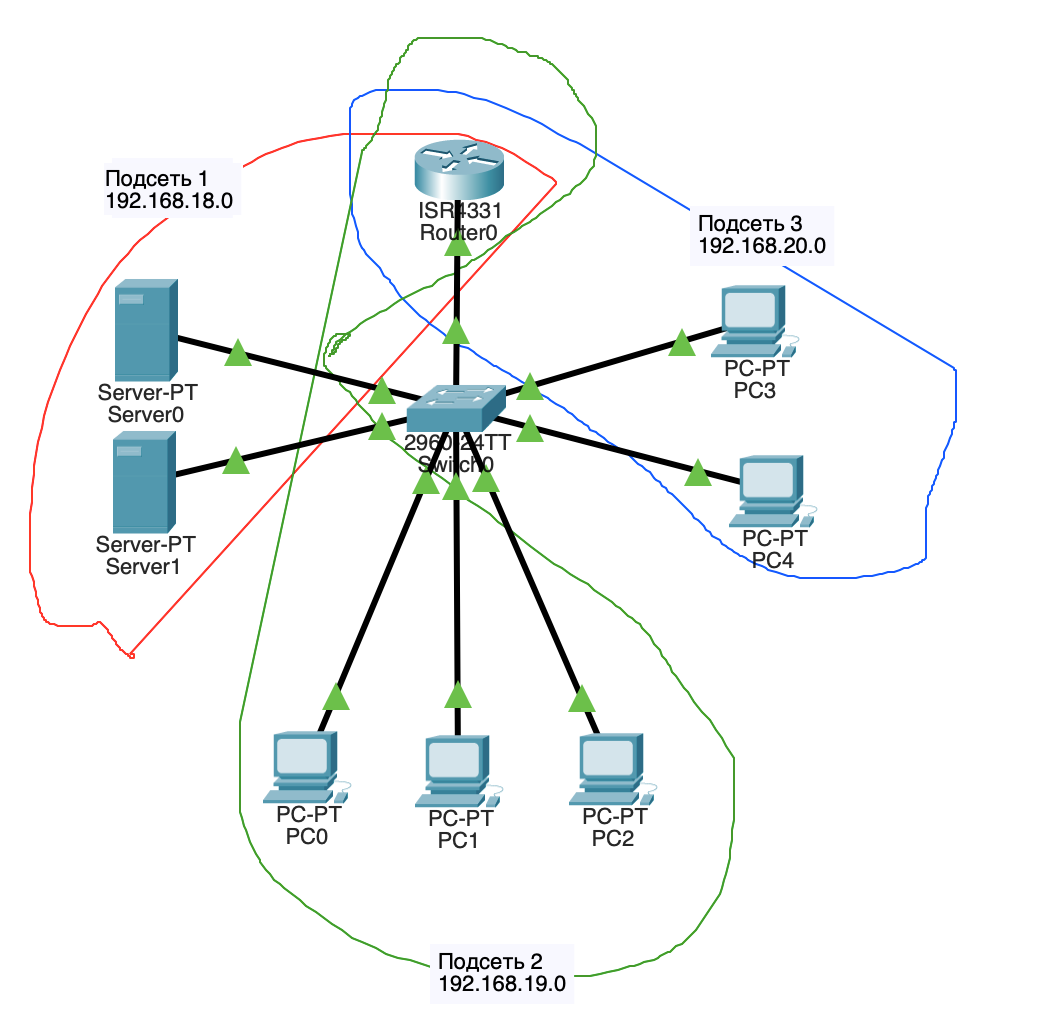
\includegraphics[scale=0.8]{9}
  \caption{Полная схема. }
\end{figure}

\begin{figure}[H]
  \centering
  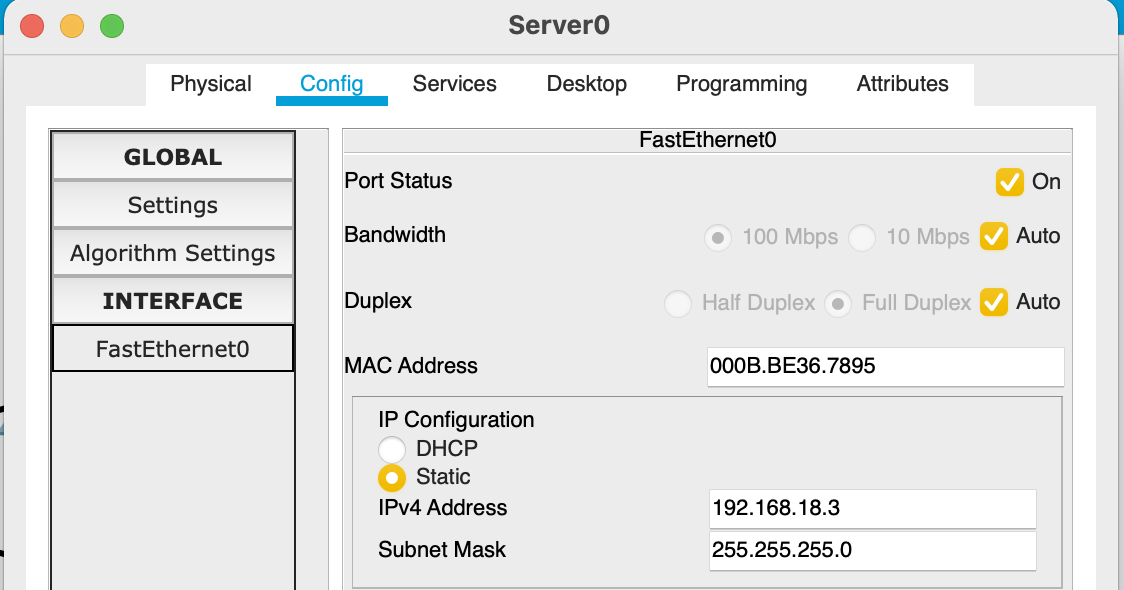
\includegraphics[scale=0.56]{5}
  \caption{IP-адрес для сервера из первой подсети. }
\end{figure}

\begin{figure}[H]
  \centering
  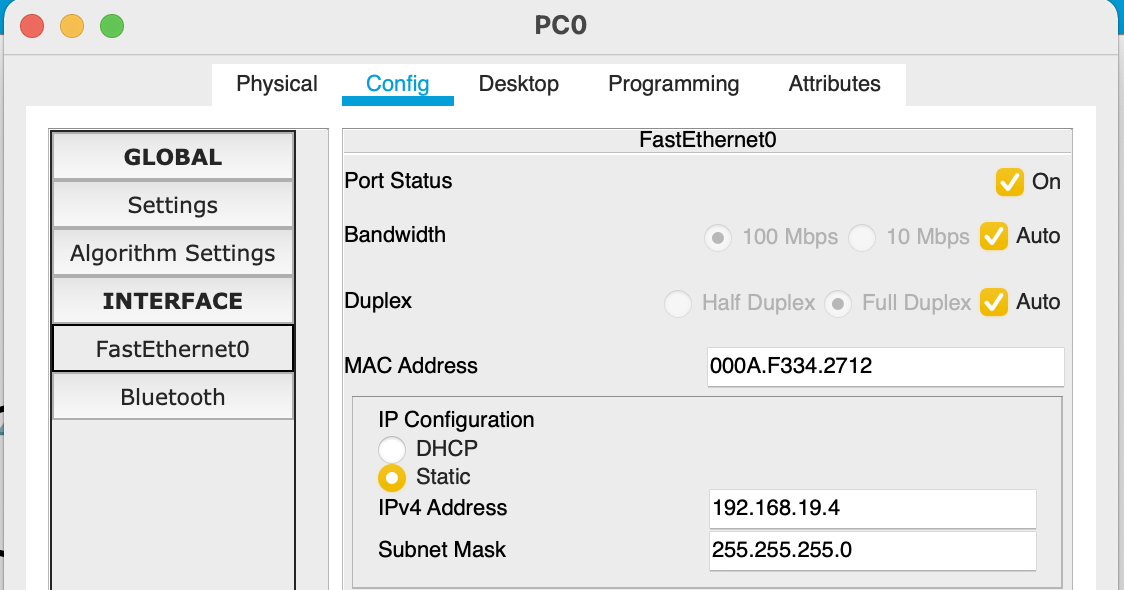
\includegraphics[scale=0.6]{6}
  \caption{IP-адрес для компьютера из второй подсети. }
\end{figure}

\begin{figure}[H]
  \centering
  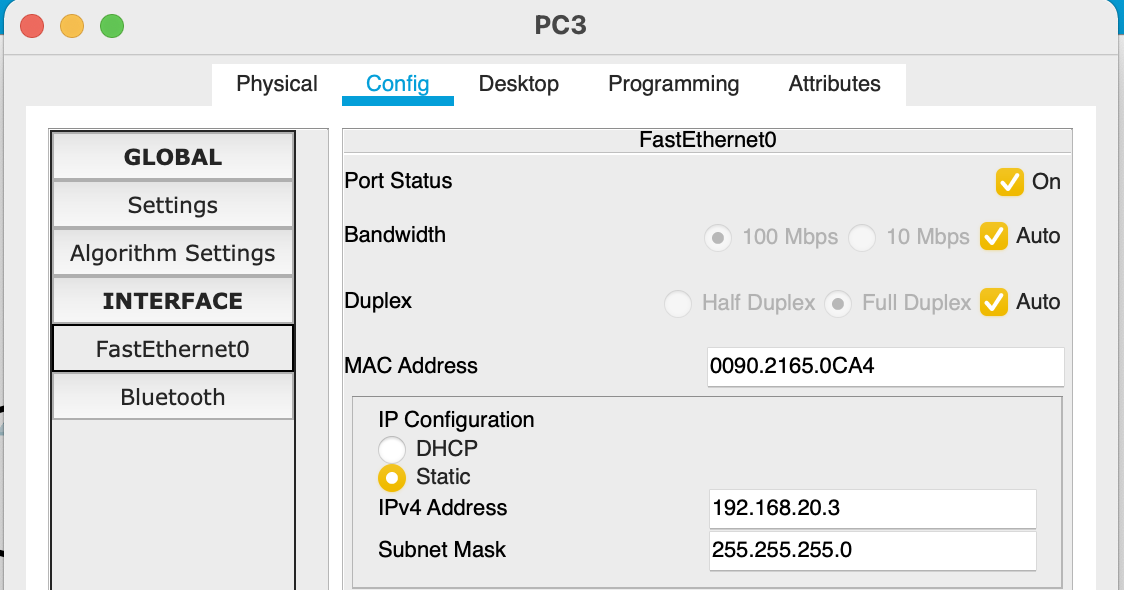
\includegraphics[scale=0.6]{7}
  \caption{IP-адрес для компьютера из третьей подсети. }
\end{figure}

\newpage
 
\item Настроить поддержку трех виртуальных локальных сетей (VLan 10, 20, 30) на коммутаторе.

Настройка для vlan 10 показана на рисунке 5, vlan 20 и 30 делаются по аналогии, результаты настройки портов приведены на рисунке 6.
 
\begin{figure}[H]
  \centering
  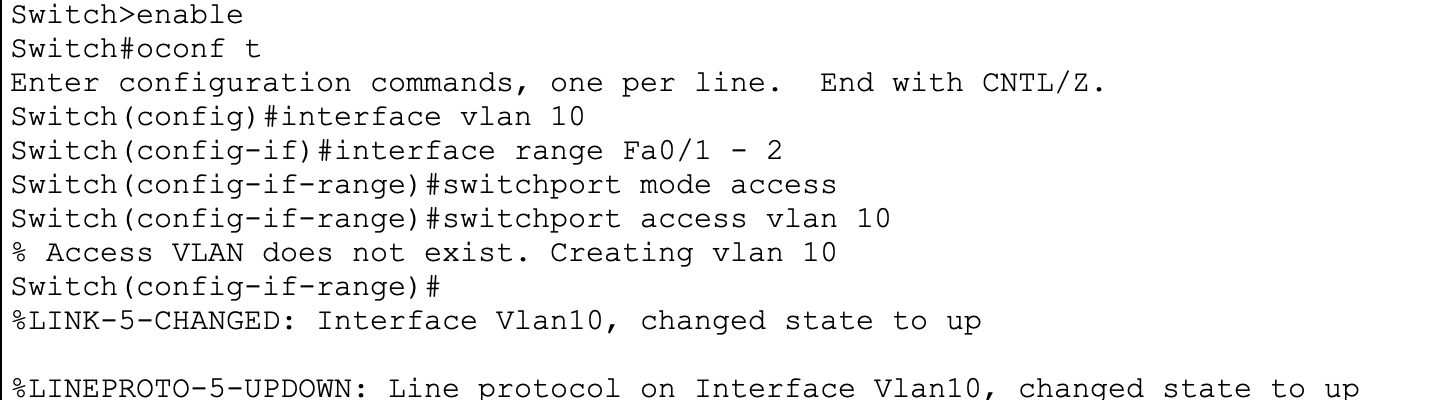
\includegraphics[scale=0.7]{1}
  \caption{Настройка vlan 10. }
\end{figure}

\begin{figure}[H]
  \centering
  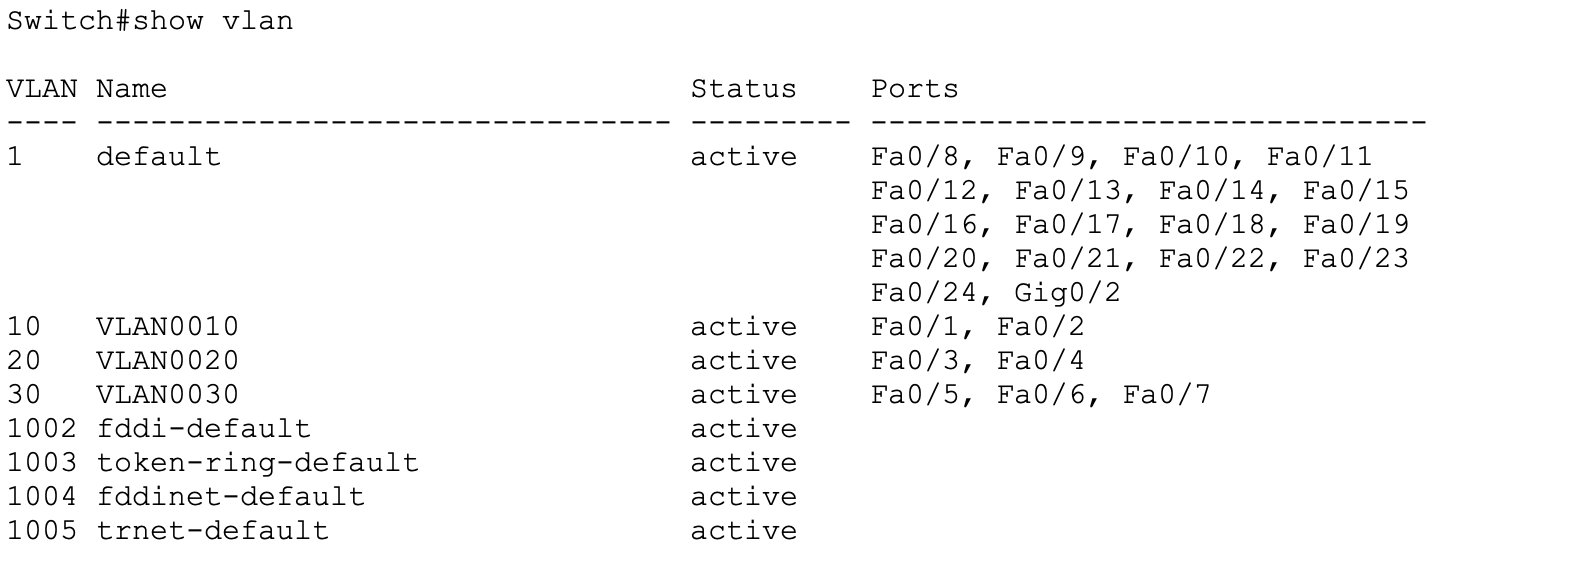
\includegraphics[scale=0.7]{4}
  \caption{Результат команды show vlan. }
\end{figure}


\item Настроить маршрутизацию между виртуальными локальными сетями на маршрутизаторе.

Так как используется общий физический канал для всех виртуальных локальных сетей, адреса шлюзов для каждой должны быть назначены виртуальным подинтерфейсам. Результат данной настройки показан на рисунке 7.

\begin{figure}[H]
  \centering
  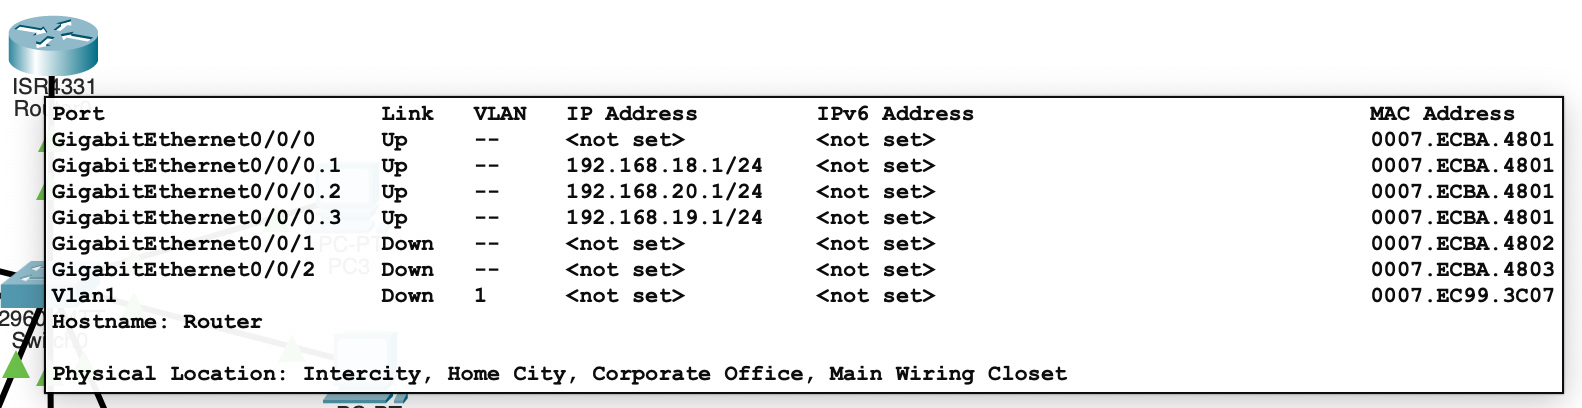
\includegraphics[scale=0.7]{8}
  \caption{Настройки роутера. }
\end{figure}

Для проверки правильной настройки маршрутизации делаем ping, представлен на рисунках 8 и 9.

\begin{figure}[H]
  \centering
  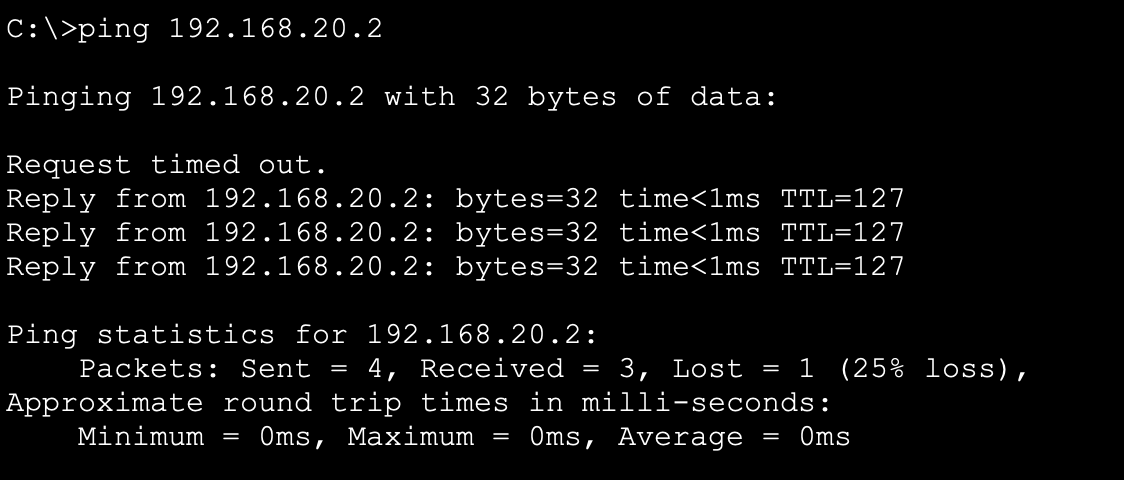
\includegraphics[scale=0.8]{11}
  \caption{Ping сервером 0 компьютера 4. }
\end{figure}

\begin{figure}[H]
  \centering
  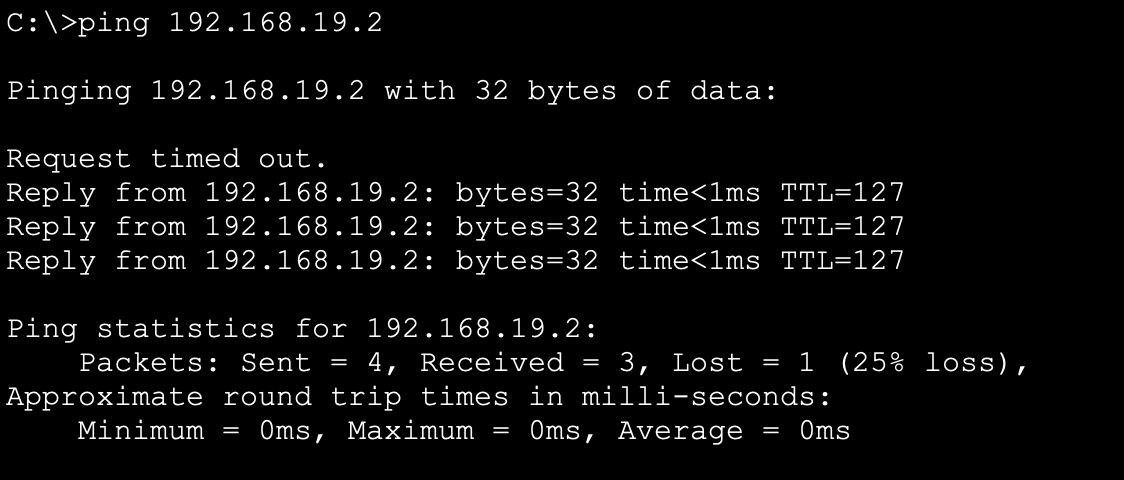
\includegraphics[scale=0.8]{12}
  \caption{Ping сервером 0 компьютера 1. }
\end{figure}

\item Выделить и озаглавить на схеме каждую виртуальную локальную сеть.

На рисунке 10 представлена схема с обозначениями каждой виртуальной сети.

\begin{figure}[H]
  \centering
  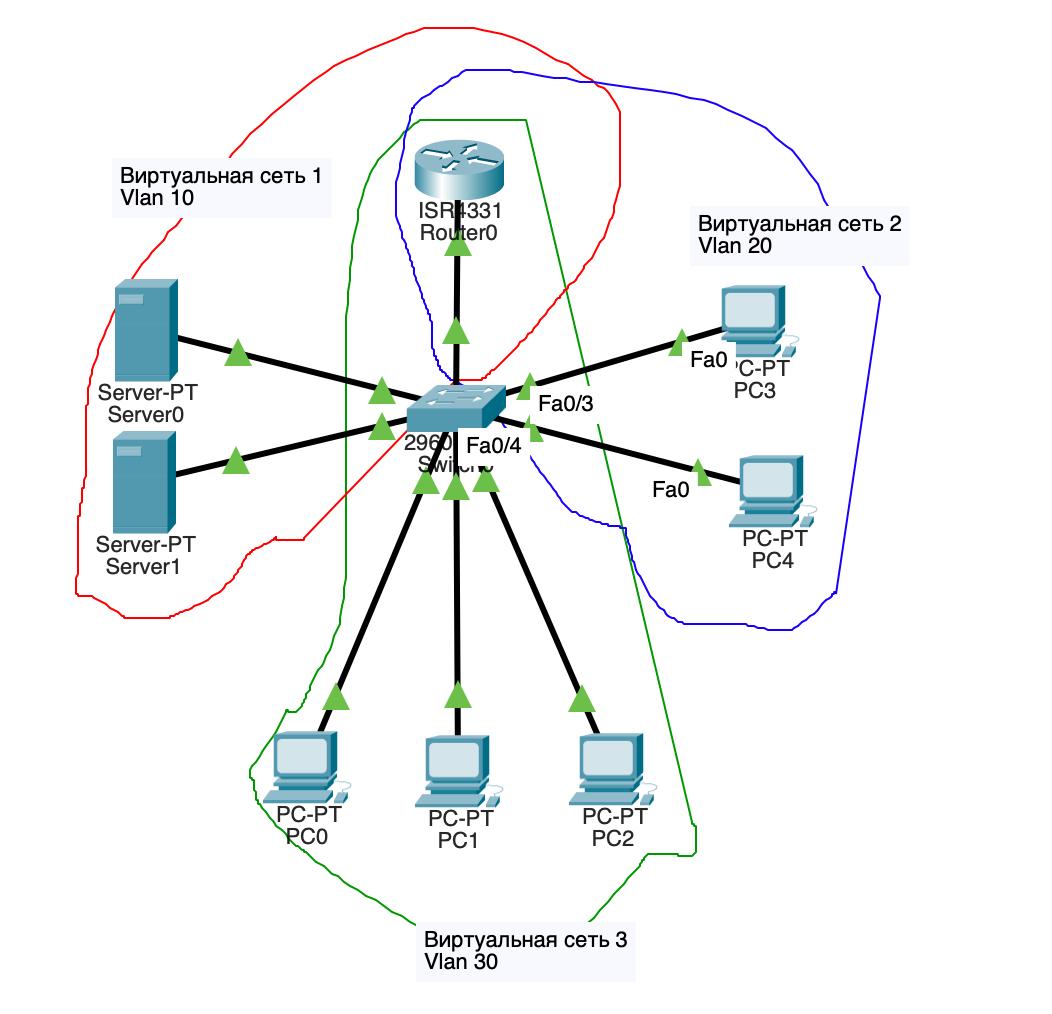
\includegraphics[scale=0.8]{10}
  \caption{Виртуальные сети. }
\end{figure}

\end{enumerate}


\end{document}